% Options for packages loaded elsewhere
\PassOptionsToPackage{unicode}{hyperref}
\PassOptionsToPackage{hyphens}{url}
%
\documentclass[
]{article}
\usepackage{lmodern}
\usepackage{amssymb,amsmath}
\usepackage{ifxetex,ifluatex}
\ifnum 0\ifxetex 1\fi\ifluatex 1\fi=0 % if pdftex
  \usepackage[T1]{fontenc}
  \usepackage[utf8]{inputenc}
  \usepackage{textcomp} % provide euro and other symbols
\else % if luatex or xetex
  \usepackage{unicode-math}
  \defaultfontfeatures{Scale=MatchLowercase}
  \defaultfontfeatures[\rmfamily]{Ligatures=TeX,Scale=1}
\fi
% Use upquote if available, for straight quotes in verbatim environments
\IfFileExists{upquote.sty}{\usepackage{upquote}}{}
\IfFileExists{microtype.sty}{% use microtype if available
  \usepackage[]{microtype}
  \UseMicrotypeSet[protrusion]{basicmath} % disable protrusion for tt fonts
}{}
\makeatletter
\@ifundefined{KOMAClassName}{% if non-KOMA class
  \IfFileExists{parskip.sty}{%
    \usepackage{parskip}
  }{% else
    \setlength{\parindent}{0pt}
    \setlength{\parskip}{6pt plus 2pt minus 1pt}}
}{% if KOMA class
  \KOMAoptions{parskip=half}}
\makeatother
\usepackage{xcolor}
\IfFileExists{xurl.sty}{\usepackage{xurl}}{} % add URL line breaks if available
\IfFileExists{bookmark.sty}{\usepackage{bookmark}}{\usepackage{hyperref}}
\hypersetup{
  pdftitle={ATLAS DEL POTENCIAL ENERGÉTICO DE OCÉANOS},
  pdfauthor={Efraín Mateos Farfán; Julio Sergio Santana; Edmundo Pedroza González},
  hidelinks,
  pdfcreator={LaTeX via pandoc}}
\urlstyle{same} % disable monospaced font for URLs
\usepackage{longtable,booktabs}
% Correct order of tables after \paragraph or \subparagraph
\usepackage{etoolbox}
\makeatletter
\patchcmd\longtable{\par}{\if@noskipsec\mbox{}\fi\par}{}{}
\makeatother
% Allow footnotes in longtable head/foot
\IfFileExists{footnotehyper.sty}{\usepackage{footnotehyper}}{\usepackage{footnote}}
\makesavenoteenv{longtable}
\usepackage{graphicx}
\makeatletter
\def\maxwidth{\ifdim\Gin@nat@width>\linewidth\linewidth\else\Gin@nat@width\fi}
\def\maxheight{\ifdim\Gin@nat@height>\textheight\textheight\else\Gin@nat@height\fi}
\makeatother
% Scale images if necessary, so that they will not overflow the page
% margins by default, and it is still possible to overwrite the defaults
% using explicit options in \includegraphics[width, height, ...]{}
\setkeys{Gin}{width=\maxwidth,height=\maxheight,keepaspectratio}
% Set default figure placement to htbp
\makeatletter
\def\fps@figure{htbp}
\makeatother
\setlength{\emergencystretch}{3em} % prevent overfull lines
\providecommand{\tightlist}{%
  \setlength{\itemsep}{0pt}\setlength{\parskip}{0pt}}
\setcounter{secnumdepth}{5}
\usepackage{booktabs}
\usepackage[spanish]{babel}
\usepackage[utf8]{inputenc}
\usepackage{url}
% \usepackage[T1]{fontenc}
\usepackage{textcomp}
% \renewcommand{\bibname}{Referencias}
\renewcommand{\refname}{Referencias}
\renewcommand\spanishtablename{Tabla}
\ifluatex
  \usepackage{selnolig}  % disable illegal ligatures
\fi
\newlength{\cslhangindent}
\setlength{\cslhangindent}{1.5em}
\newenvironment{cslreferences}%
  {\setlength{\parindent}{0pt}%
  \everypar{\setlength{\hangindent}{\cslhangindent}}\ignorespaces}%
  {\par}

\title{ATLAS DEL POTENCIAL ENERGÉTICO DE OCÉANOS}
\usepackage{etoolbox}
\makeatletter
\providecommand{\subtitle}[1]{% add subtitle to \maketitle
  \apptocmd{\@title}{\par {\large #1 \par}}{}{}
}
\makeatother
\subtitle{Plantilla para la generación de libros interactivos con contenidos gráficos y numéricos}
\author{Efraín Mateos Farfán \and Julio Sergio Santana \and Edmundo Pedroza González}
\date{2020-10-05}

\begin{document}
\maketitle

{
\setcounter{tocdepth}{2}
\tableofcontents
}
\hypertarget{pruxf3logo}{%
\section{Prólogo}\label{pruxf3logo}}

Lorem ipsum dolor sit amet, consectetur adipiscing elit. Vivamus sollicitudin suscipit varius. Cras sit amet magna in arcu pretium malesuada non et tortor. Suspendisse potenti. Pellentesque eu ullamcorper velit, eu gravida risus. Aliquam fermentum tellus ac velit rhoncus efficitur ac eu dui. Proin urna arcu, tempus a sagittis volutpat, rutrum sed ex. Ut tempus quis ligula vitae aliquam.

Pellentesque habitant morbi tristique senectus et netus et malesuada fames ac turpis egestas. In fermentum scelerisque dui, ac volutpat nisl aliquam at. Donec dui urna, posuere egestas ligula vel, fringilla ultrices erat. Phasellus molestie fringilla massa, ac ultrices libero facilisis quis. In volutpat molestie dapibus. Vivamus non nunc nec ex elementum facilisis. Donec in purus ex. Donec interdum sollicitudin nunc ut luctus. Mauris vel finibus est, id lobortis nulla. Vestibulum ante ipsum primis in faucibus orci luctus et ultrices posuere cubilia curae; Quisque vulputate, dui sed molestie lacinia, metus ipsum volutpat odio, vitae tincidunt urna nulla quis purus. Sed posuere ex in magna ullamcorper, sit amet interdum metus venenatis.

Nullam eget lobortis urna. Maecenas ipsum lorem, cursus nec dui ut, malesuada aliquam neque. Cras quis laoreet ipsum. Donec imperdiet, diam at laoreet iaculis, nisi sapien efficitur ligula, convallis fermentum nulla velit in ipsum. Cras non aliquam augue. Curabitur ac odio eros. Mauris id condimentum augue, sed rhoncus orci. In hac habitasse platea dictumst. Vivamus viverra nisl efficitur dapibus aliquam. Vivamus fringilla, felis eu porttitor congue, orci est pulvinar eros, vitae consectetur tellus enim non urna. Suspendisse pharetra vel felis id fringilla.

Sed ex neque, egestas et sodales sed, viverra vel sem. Duis sollicitudin justo vitae dignissim dignissim. Pellentesque faucibus, tellus eget facilisis pulvinar, odio libero dapibus risus, sed vulputate orci metus vitae eros. Curabitur maximus neque in dui tempus facilisis. Vivamus sed eleifend nisi. Mauris accumsan turpis justo, et elementum enim porta nec. Aliquam rhoncus metus sed tortor pharetra, blandit bibendum metus pretium. Vivamus iaculis, dolor quis scelerisque fringilla, est lectus mollis ante, at pulvinar sapien augue sed nisi. Praesent auctor varius orci, non pharetra nunc mollis ut. Duis vulputate sodales erat, tristique sagittis libero consectetur facilisis. Donec id sapien auctor, imperdiet mauris a, volutpat tellus. Fusce non lorem eget libero pulvinar semper.

Donec consequat maximus nunc, sed porttitor neque aliquet sed. In consectetur, mi sed faucibus laoreet, ex sem congue leo, eu maximus purus nisl at nunc. Quisque iaculis vehicula quam, a dictum nisl rutrum ut. Vestibulum varius gravida congue. Ut fermentum elementum libero, in malesuada sapien tempor et. Suspendisse tellus eros, placerat id velit id, tempus condimentum mi. Sed sem turpis, venenatis id sodales ut, porta vitae nibh. Donec suscipit porta lacus eu blandit.

\hypertarget{intro}{%
\section{Introducción}\label{intro}}

El Centro Mexicano de Innovación en Energía Océano (CEMIE-Océano), reune a un número importante de centros de investigación. Su misión es generar productos, técnicas y tecnologías innovadoras que exploten la diversidad de recursos energéticos océanicos disponibles para suministrar de manera sustentable y rentable una parte cada vez mayor de la demanda energética de la República Mexicana.

Desde su creación, hace más de dos años, el CEMIE-Océano ha generado una gran cantidad de información, producto de las investigaciones y trabajos realizados. Esta información debe ser divulgada para permitir la vinculación entre los generadores de información con sectores de índole económica o industrial. Por la naturaleza de la información generada, gran cantidad de ésta puede ser presentada como libros tipo atlas.

\hypertarget{subsecciuxf3n-para-incluir-referencias}{%
\subsection{Subsección para incluir referencias}\label{subsecciuxf3n-para-incluir-referencias}}

En el objetivo se hace referencia a \emph{libros con contenidos gráficos y numéricos en forma de atlas interactivos}, lo que es una especialización del concepto más general: \emph{libros digitales interactivos}. El concepto de libros interactivos tiene su origen en los libros \emph{pop-up} para niños, creados por Julian Wehr en la década de 1940 (Boehm \& Ziegler, \protect\hyperlink{ref-Bohem2002}{2002}; Movable Book Society, \protect\hyperlink{ref-MBS2002}{2002}). Estos libros tangibles, permiten a los niños interactuar con su contenido, mediante el accionar de las pestañas de papel o cartón, provistas en el libro para \emph{animar} o dar movilidad a las ilustraciones, tal como el que se muestra en la animación de abajo. Más tarde, con el advenimiento de los libros digitales o electrónicos, los portales \emph{Web} y los libros en línea (Reilly, \protect\hyperlink{ref-Reilly2003}{2003}), la idea de que los lectores pudieran interactuar con su contenido permeó de los libros tangibles a los libros digitales en línea.

\hypertarget{oceano-pacuxedfico}{%
\section{Oceano Pacífico}\label{oceano-pacuxedfico}}

Lorem ipsum dolor sit amet, consectetur adipiscing elit. Vivamus sollicitudin suscipit varius. Cras sit amet magna in arcu pretium malesuada non et tortor. Suspendisse potenti. Pellentesque eu ullamcorper velit, eu gravida risus. Aliquam fermentum tellus ac velit rhoncus efficitur ac eu dui. Proin urna arcu, tempus a sagittis volutpat, rutrum sed ex. Ut tempus quis ligula vitae aliquam.

Pellentesque habitant morbi tristique senectus et netus et malesuada fames ac turpis egestas. In fermentum scelerisque dui, ac volutpat nisl aliquam at. Donec dui urna, posuere egestas ligula vel, fringilla ultrices erat. Phasellus molestie fringilla massa, ac ultrices libero facilisis quis. In volutpat molestie dapibus. Vivamus non nunc nec ex elementum facilisis. Donec in purus ex. Donec interdum sollicitudin nunc ut luctus. Mauris vel finibus est, id lobortis nulla. Vestibulum ante ipsum primis in faucibus orci luctus et ultrices posuere cubilia curae; Quisque vulputate, dui sed molestie lacinia, metus ipsum volutpat odio, vitae tincidunt urna nulla quis purus. Sed posuere ex in magna ullamcorper, sit amet interdum metus venenatis.

\hypertarget{rapidez-y-velocidad-en-el-ocuxe9ano}{%
\subsection{Rapidez y velocidad en el océano}\label{rapidez-y-velocidad-en-el-ocuxe9ano}}

Pellentesque habitant morbi tristique senectus et netus et malesuada fames ac turpis egestas. In fermentum scelerisque dui, ac volutpat nisl aliquam at. Donec dui urna, posuere egestas ligula vel, fringilla ultrices erat. Phasellus molestie fringilla massa, ac ultrices libero facilisis quis. In volutpat molestie dapibus. Vivamus non nunc nec ex elementum facilisis. Donec in purus ex. Donec interdum sollicitudin nunc ut luctus. Mauris vel finibus est, id lobortis nulla. Vestibulum ante ipsum primis in faucibus orci luctus et ultrices posuere cubilia curae; Quisque vulputate, dui sed molestie lacinia, metus ipsum volutpat odio, vitae tincidunt urna nulla quis purus. Sed posuere ex in magna ullamcorper, sit amet interdum metus venenatis.

\begin{figure}
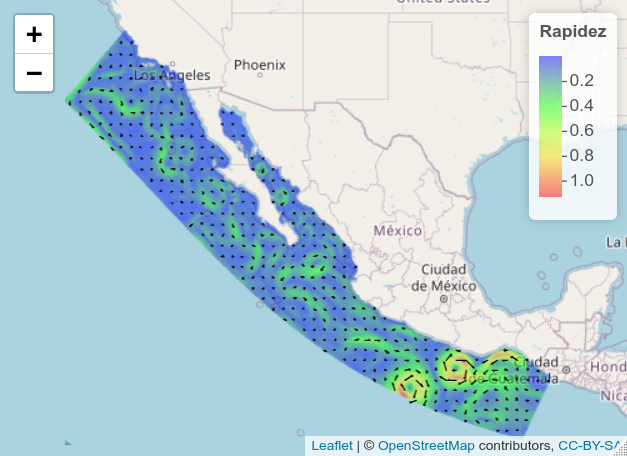
\includegraphics[width=0.95\linewidth]{images/pacifico01} \caption{Rapidez y velociad de corriente en el Pacífico}\label{fig:Mapa01}
\end{figure}

A continuación se da una breve descripción de los elementos mostrados en la Figura \ref{fig:Mapa01}.

Nullam eget lobortis urna. Maecenas ipsum lorem, cursus nec dui ut, malesuada aliquam neque. Cras quis laoreet ipsum. Donec imperdiet, diam at laoreet iaculis, nisi sapien efficitur ligula, convallis fermentum nulla velit in ipsum. Cras non aliquam augue. Curabitur ac odio eros. Mauris id condimentum augue, sed rhoncus orci. In hac habitasse platea dictumst. Vivamus viverra nisl efficitur dapibus aliquam. Vivamus fringilla, felis eu porttitor congue, orci est pulvinar eros, vitae consectetur tellus enim non urna. Suspendisse pharetra vel felis id fringilla.

Sed ex neque, egestas et sodales sed, viverra vel sem. Duis sollicitudin justo vitae dignissim dignissim. Pellentesque faucibus, tellus eget facilisis pulvinar, odio libero dapibus risus, sed vulputate orci metus vitae eros. Curabitur maximus neque in dui tempus facilisis. Vivamus sed eleifend nisi. Mauris accumsan turpis justo, et elementum enim porta nec. Aliquam rhoncus metus sed tortor pharetra, blandit bibendum metus pretium. Vivamus iaculis, dolor quis scelerisque fringilla, est lectus mollis ante, at pulvinar sapien augue sed nisi. Praesent auctor varius orci, non pharetra nunc mollis ut. Duis vulputate sodales erat, tristique sagittis libero consectetur facilisis. Donec id sapien auctor, imperdiet mauris a, volutpat tellus. Fusce non lorem eget libero pulvinar semper.

Donec consequat maximus nunc, sed porttitor neque aliquet sed. In consectetur, mi sed faucibus laoreet, ex sem congue leo, eu maximus purus nisl at nunc. Quisque iaculis vehicula quam, a dictum nisl rutrum ut. Vestibulum varius gravida congue. Ut fermentum elementum libero, in malesuada sapien tempor et. Suspendisse tellus eros, placerat id velit id, tempus condimentum mi. Sed sem turpis, venenatis id sodales ut, porta vitae nibh. Donec suscipit porta lacus eu blandit.

\hypertarget{otras-variables-en-el-ocuxe9ano}{%
\subsection{Otras variables en el océano}\label{otras-variables-en-el-ocuxe9ano}}

Pellentesque habitant morbi tristique senectus et netus et malesuada fames ac turpis egestas. In fermentum scelerisque dui, ac volutpat nisl aliquam at. Donec dui urna, posuere egestas ligula vel, fringilla ultrices erat. Phasellus molestie fringilla massa, ac ultrices libero facilisis quis. In volutpat molestie dapibus. Vivamus non nunc nec ex elementum facilisis. Donec in purus ex. Donec interdum sollicitudin nunc ut luctus. Mauris vel finibus est, id lobortis nulla. Vestibulum ante ipsum primis in faucibus orci luctus et ultrices posuere cubilia curae; Quisque vulputate, dui sed molestie lacinia, metus ipsum volutpat odio, vitae tincidunt urna nulla quis purus. Sed posuere ex in magna ullamcorper, sit amet interdum metus venenatis.

\begin{figure}
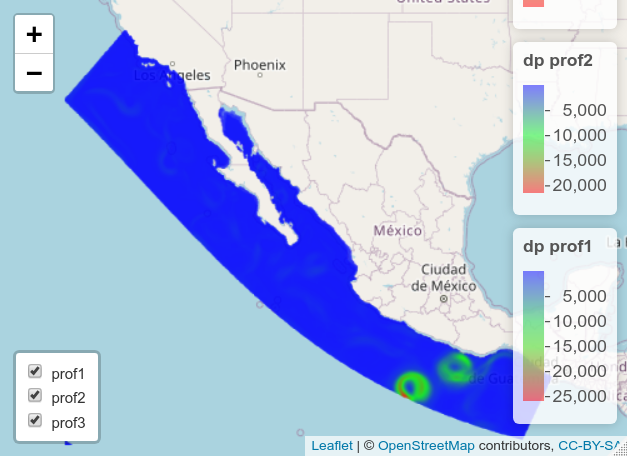
\includegraphics[width=0.95\linewidth]{images/dp01} \caption{Variable dp en el Pacífico a distintas profundidaes}\label{fig:Mapa02}
\end{figure}

Pellentesque habitant morbi tristique senectus et netus et malesuada fames ac turpis egestas. In fermentum scelerisque dui, ac volutpat nisl aliquam at. Donec dui urna, posuere egestas ligula vel, fringilla ultrices erat. Phasellus molestie fringilla massa, ac ultrices libero facilisis quis. In volutpat molestie dapibus. Vivamus non nunc nec ex elementum facilisis. Donec in purus ex. Donec interdum sollicitudin nunc ut luctus. Mauris vel finibus est, id lobortis nulla. Vestibulum ante ipsum primis in faucibus orci luctus et ultrices posuere cubilia curae; Quisque vulputate, dui sed molestie lacinia, metus ipsum volutpat odio, vitae tincidunt urna nulla quis purus. Sed posuere ex in magna ullamcorper, sit amet interdum metus venenatis.

\hypertarget{golfo-de-muxe9xico}{%
\section{Golfo de México}\label{golfo-de-muxe9xico}}

\hypertarget{rapidez-y-velocidad-en-el-golfo-de-muxe9xico}{%
\subsection{Rapidez y velocidad en el Golfo de México}\label{rapidez-y-velocidad-en-el-golfo-de-muxe9xico}}

Lorem ipsum dolor sit amet, consectetur adipiscing elit. Vivamus sollicitudin suscipit varius. Cras sit amet magna in arcu pretium malesuada non et tortor. Suspendisse potenti. Pellentesque eu ullamcorper velit, eu gravida risus. Aliquam fermentum tellus ac velit rhoncus efficitur ac eu dui. Proin urna arcu, tempus a sagittis volutpat, rutrum sed ex. Ut tempus quis ligula vitae aliquam.

\begin{figure}
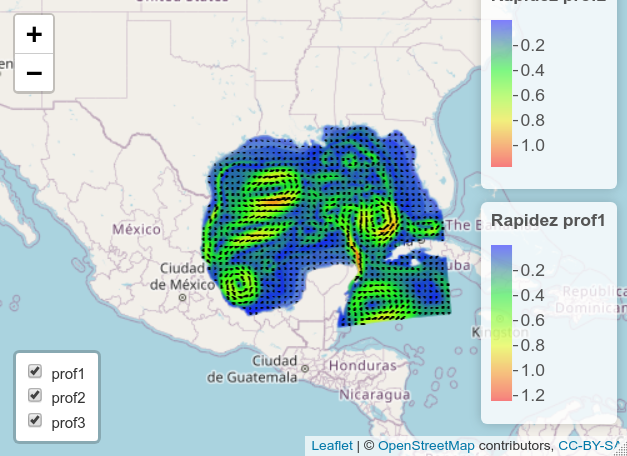
\includegraphics[width=0.95\linewidth]{images/golfomex01} \caption{Rapidez y velociad de corriente en el Golfo de México}\label{fig:Mapa03}
\end{figure}

Pellentesque habitant morbi tristique senectus et netus et malesuada fames ac turpis egestas. In fermentum scelerisque dui, ac volutpat nisl aliquam at. Donec dui urna, posuere egestas ligula vel, fringilla ultrices erat. Phasellus molestie fringilla massa, ac ultrices libero facilisis quis. In volutpat molestie dapibus. Vivamus non nunc nec ex elementum facilisis. Donec in purus ex. Donec interdum sollicitudin nunc ut luctus. Mauris vel finibus est, id lobortis nulla. Vestibulum ante ipsum primis in faucibus orci luctus et ultrices posuere cubilia curae; Quisque vulputate, dui sed molestie lacinia, metus ipsum volutpat odio, vitae tincidunt urna nulla quis purus. Sed posuere ex in magna ullamcorper, sit amet interdum metus venenatis.

Nullam eget lobortis urna. Maecenas ipsum lorem, cursus nec dui ut, malesuada aliquam neque. Cras quis laoreet ipsum. Donec imperdiet, diam at laoreet iaculis, nisi sapien efficitur ligula, convallis fermentum nulla velit in ipsum. Cras non aliquam augue. Curabitur ac odio eros. Mauris id condimentum augue, sed rhoncus orci. In hac habitasse platea dictumst. Vivamus viverra nisl efficitur dapibus aliquam. Vivamus fringilla, felis eu porttitor congue, orci est pulvinar eros, vitae consectetur tellus enim non urna. Suspendisse pharetra vel felis id fringilla.

Sed ex neque, egestas et sodales sed, viverra vel sem. Duis sollicitudin justo vitae dignissim dignissim. Pellentesque faucibus, tellus eget facilisis pulvinar, odio libero dapibus risus, sed vulputate orci metus vitae eros. Curabitur maximus neque in dui tempus facilisis. Vivamus sed eleifend nisi. Mauris accumsan turpis justo, et elementum enim porta nec. Aliquam rhoncus metus sed tortor pharetra, blandit bibendum metus pretium. Vivamus iaculis, dolor quis scelerisque fringilla, est lectus mollis ante, at pulvinar sapien augue sed nisi. Praesent auctor varius orci, non pharetra nunc mollis ut. Duis vulputate sodales erat, tristique sagittis libero consectetur facilisis. Donec id sapien auctor, imperdiet mauris a, volutpat tellus. Fusce non lorem eget libero pulvinar semper.

\hypertarget{otras-variables-en-el-golfo-de-muxe9xico}{%
\subsection{Otras variables en el Golfo de México}\label{otras-variables-en-el-golfo-de-muxe9xico}}

Donec consequat maximus nunc, sed porttitor neque aliquet sed. In consectetur, mi sed faucibus laoreet, ex sem congue leo, eu maximus purus nisl at nunc. Quisque iaculis vehicula quam, a dictum nisl rutrum ut. Vestibulum varius gravida congue. Ut fermentum elementum libero, in malesuada sapien tempor et. Suspendisse tellus eros, placerat id velit id, tempus condimentum mi. Sed sem turpis, venenatis id sodales ut, porta vitae nibh. Donec suscipit porta lacus eu blandit.

Pellentesque habitant morbi tristique senectus et netus et malesuada fames ac turpis egestas. In fermentum scelerisque dui, ac volutpat nisl aliquam at. Donec dui urna, posuere egestas ligula vel, fringilla ultrices erat. Phasellus molestie fringilla massa, ac ultrices libero facilisis quis. In volutpat molestie dapibus. Vivamus non nunc nec ex elementum facilisis. Donec in purus ex. Donec interdum sollicitudin nunc ut luctus. Mauris vel finibus est, id lobortis nulla. Vestibulum ante ipsum primis in faucibus orci luctus et ultrices posuere cubilia curae; Quisque vulputate, dui sed molestie lacinia, metus ipsum volutpat odio, vitae tincidunt urna nulla quis purus. Sed posuere ex in magna ullamcorper, sit amet interdum metus venenatis.

\begin{figure}
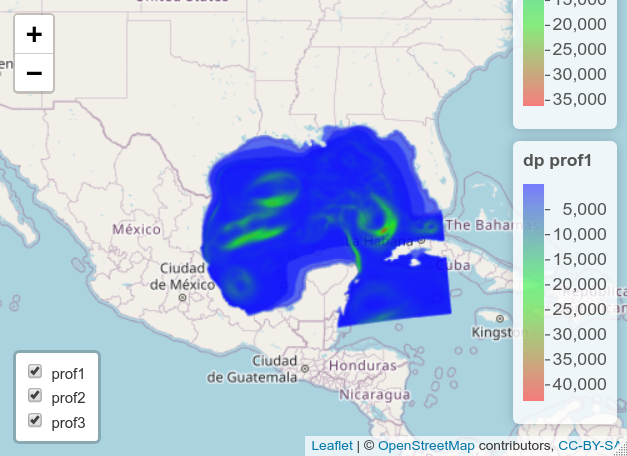
\includegraphics[width=0.95\linewidth]{images/golfomex02} \caption{Variable dp en el Golfo de México}\label{fig:Mapa04}
\end{figure}

Lorem ipsum dolor sit amet, consectetur adipiscing elit. Vivamus sollicitudin suscipit varius. Cras sit amet magna in arcu pretium malesuada non et tortor. Suspendisse potenti. Pellentesque eu ullamcorper velit, eu gravida risus. Aliquam fermentum tellus ac velit rhoncus efficitur ac eu dui. Proin urna arcu, tempus a sagittis volutpat, rutrum sed ex. Ut tempus quis ligula vitae aliquam.

Pellentesque habitant morbi tristique senectus et netus et malesuada fames ac turpis egestas. In fermentum scelerisque dui, ac volutpat nisl aliquam at. Donec dui urna, posuere egestas ligula vel, fringilla ultrices erat. Phasellus molestie fringilla massa, ac ultrices libero facilisis quis. In volutpat molestie dapibus. Vivamus non nunc nec ex elementum facilisis. Donec in purus ex. Donec interdum sollicitudin nunc ut luctus. Mauris vel finibus est, id lobortis nulla. Vestibulum ante ipsum primis in faucibus orci luctus et ultrices posuere cubilia curae; Quisque vulputate, dui sed molestie lacinia, metus ipsum volutpat odio, vitae tincidunt urna nulla quis purus. Sed posuere ex in magna ullamcorper, sit amet interdum metus venenatis.

Nullam eget lobortis urna. Maecenas ipsum lorem, cursus nec dui ut, malesuada aliquam neque. Cras quis laoreet ipsum. Donec imperdiet, diam at laoreet iaculis, nisi sapien efficitur ligula, convallis fermentum nulla velit in ipsum. Cras non aliquam augue. Curabitur ac odio eros. Mauris id condimentum augue, sed rhoncus orci. In hac habitasse platea dictumst. Vivamus viverra nisl efficitur dapibus aliquam. Vivamus fringilla, felis eu porttitor congue, orci est pulvinar eros, vitae consectetur tellus enim non urna. Suspendisse pharetra vel felis id fringilla.

Sed ex neque, egestas et sodales sed, viverra vel sem. Duis sollicitudin justo vitae dignissim dignissim. Pellentesque faucibus, tellus eget facilisis pulvinar, odio libero dapibus risus, sed vulputate orci metus vitae eros. Curabitur maximus neque in dui tempus facilisis. Vivamus sed eleifend nisi. Mauris accumsan turpis justo, et elementum enim porta nec. Aliquam rhoncus metus sed tortor pharetra, blandit bibendum metus pretium. Vivamus iaculis, dolor quis scelerisque fringilla, est lectus mollis ante, at pulvinar sapien augue sed nisi. Praesent auctor varius orci, non pharetra nunc mollis ut. Duis vulputate sodales erat, tristique sagittis libero consectetur facilisis. Donec id sapien auctor, imperdiet mauris a, volutpat tellus. Fusce non lorem eget libero pulvinar semper.

Donec consequat maximus nunc, sed porttitor neque aliquet sed. In consectetur, mi sed faucibus laoreet, ex sem congue leo, eu maximus purus nisl at nunc. Quisque iaculis vehicula quam, a dictum nisl rutrum ut. Vestibulum varius gravida congue. Ut fermentum elementum libero, in malesuada sapien tempor et. Suspendisse tellus eros, placerat id velit id, tempus condimentum mi. Sed sem turpis, venenatis id sodales ut, porta vitae nibh. Donec suscipit porta lacus eu blandit.

\hypertarget{golfo-de-california}{%
\section{Golfo de California}\label{golfo-de-california}}

Lorem ipsum dolor sit amet, consectetur adipiscing elit. Vivamus sollicitudin suscipit varius. Cras sit amet magna in arcu pretium malesuada non et tortor. Suspendisse potenti. Pellentesque eu ullamcorper velit, eu gravida risus. Aliquam fermentum tellus ac velit rhoncus efficitur ac eu dui. Proin urna arcu, tempus a sagittis volutpat, rutrum sed ex. Ut tempus quis ligula vitae aliquam.

Pellentesque habitant morbi tristique senectus et netus et malesuada fames ac turpis egestas. In fermentum scelerisque dui, ac volutpat nisl aliquam at. Donec dui urna, posuere egestas ligula vel, fringilla ultrices erat. Phasellus molestie fringilla massa, ac ultrices libero facilisis quis. In volutpat molestie dapibus. Vivamus non nunc nec ex elementum facilisis. Donec in purus ex. Donec interdum sollicitudin nunc ut luctus. Mauris vel finibus est, id lobortis nulla. Vestibulum ante ipsum primis in faucibus orci luctus et ultrices posuere cubilia curae; Quisque vulputate, dui sed molestie lacinia, metus ipsum volutpat odio, vitae tincidunt urna nulla quis purus. Sed posuere ex in magna ullamcorper, sit amet interdum metus venenatis.

Nullam eget lobortis urna. Maecenas ipsum lorem, cursus nec dui ut, malesuada aliquam neque. Cras quis laoreet ipsum. Donec imperdiet, diam at laoreet iaculis, nisi sapien efficitur ligula, convallis fermentum nulla velit in ipsum. Cras non aliquam augue. Curabitur ac odio eros. Mauris id condimentum augue, sed rhoncus orci. In hac habitasse platea dictumst. Vivamus viverra nisl efficitur dapibus aliquam. Vivamus fringilla, felis eu porttitor congue, orci est pulvinar eros, vitae consectetur tellus enim non urna. Suspendisse pharetra vel felis id fringilla.

\hypertarget{algunas-variables-en-el-golfo-de-california}{%
\subsection{Algunas variables en el Golfo de California}\label{algunas-variables-en-el-golfo-de-california}}

Lorem ipsum dolor sit amet, consectetur adipiscing elit. Vivamus sollicitudin suscipit varius. Cras sit amet magna in arcu pretium malesuada non et tortor. Suspendisse potenti. Pellentesque eu ullamcorper velit, eu gravida risus. Aliquam fermentum tellus ac velit rhoncus efficitur ac eu dui. Proin urna arcu, tempus a sagittis volutpat, rutrum sed ex. Ut tempus quis ligula vitae aliquam.

Pellentesque habitant morbi tristique senectus et netus et malesuada fames ac turpis egestas. In fermentum scelerisque dui, ac volutpat nisl aliquam at. Donec dui urna, posuere egestas ligula vel, fringilla ultrices erat. Phasellus molestie fringilla massa, ac ultrices libero facilisis quis. In volutpat molestie dapibus. Vivamus non nunc nec ex elementum facilisis. Donec in purus ex. Donec interdum sollicitudin nunc ut luctus. Mauris vel finibus est, id lobortis nulla. Vestibulum ante ipsum primis in faucibus orci luctus et ultrices posuere cubilia curae; Quisque vulputate, dui sed molestie lacinia, metus ipsum volutpat odio, vitae tincidunt urna nulla quis purus. Sed posuere ex in magna ullamcorper, sit amet interdum metus venenatis.

\begin{figure}
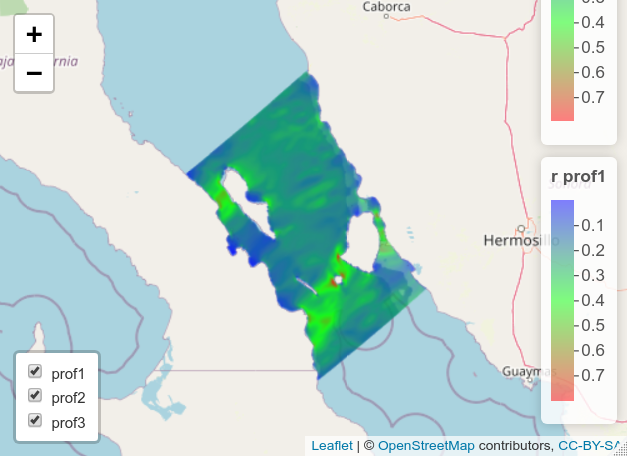
\includegraphics[width=0.95\linewidth]{images/golfocalif01} \caption{Variable r en el Golfo de California}\label{fig:Mapa05}
\end{figure}

Nullam eget lobortis urna. Maecenas ipsum lorem, cursus nec dui ut, malesuada aliquam neque. Cras quis laoreet ipsum. Donec imperdiet, diam at laoreet iaculis, nisi sapien efficitur ligula, convallis fermentum nulla velit in ipsum. Cras non aliquam augue. Curabitur ac odio eros. Mauris id condimentum augue, sed rhoncus orci. In hac habitasse platea dictumst. Vivamus viverra nisl efficitur dapibus aliquam. Vivamus fringilla, felis eu porttitor congue, orci est pulvinar eros, vitae consectetur tellus enim non urna. Suspendisse pharetra vel felis id fringilla.

Sed ex neque, egestas et sodales sed, viverra vel sem. Duis sollicitudin justo vitae dignissim dignissim. Pellentesque faucibus, tellus eget facilisis pulvinar, odio libero dapibus risus, sed vulputate orci metus vitae eros. Curabitur maximus neque in dui tempus facilisis. Vivamus sed eleifend nisi. Mauris accumsan turpis justo, et elementum enim porta nec. Aliquam rhoncus metus sed tortor pharetra, blandit bibendum metus pretium. Vivamus iaculis, dolor quis scelerisque fringilla, est lectus mollis ante, at pulvinar sapien augue sed nisi. Praesent auctor varius orci, non pharetra nunc mollis ut. Duis vulputate sodales erat, tristique sagittis libero consectetur facilisis. Donec id sapien auctor, imperdiet mauris a, volutpat tellus. Fusce non lorem eget libero pulvinar semper.

\begin{figure}
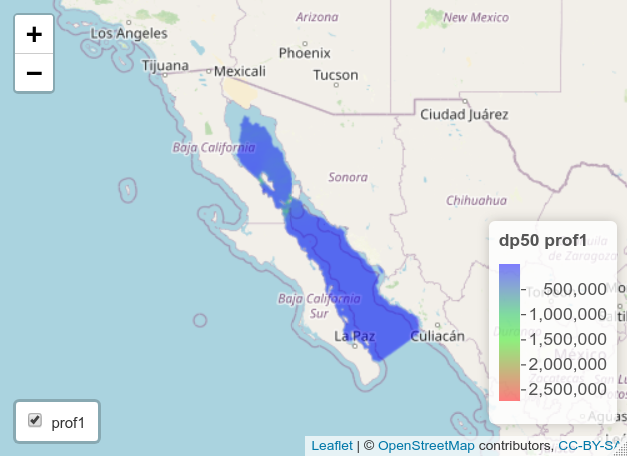
\includegraphics[width=0.95\linewidth]{images/golfocalif02} \caption{Variable dp50 en el Golfo de California}\label{fig:Mapa06}
\end{figure}

Donec consequat maximus nunc, sed porttitor neque aliquet sed. In consectetur, mi sed faucibus laoreet, ex sem congue leo, eu maximus purus nisl at nunc. Quisque iaculis vehicula quam, a dictum nisl rutrum ut. Vestibulum varius gravida congue. Ut fermentum elementum libero, in malesuada sapien tempor et. Suspendisse tellus eros, placerat id velit id, tempus condimentum mi. Sed sem turpis, venenatis id sodales ut, porta vitae nibh. Donec suscipit porta lacus eu blandit.

\hypertarget{final-words}{%
\section{Final Words}\label{final-words}}

We have finished a nice book.

\hypertarget{referencias}{%
\section*{Referencias}\label{referencias}}
\addcontentsline{toc}{section}{Referencias}

\hypertarget{refs}{}
\begin{cslreferences}
\leavevmode\hypertarget{ref-Bohem2002}{}%
Boehm, A., \& Ziegler, R. (2002). A Julian Wehr miscellany: Unrecorded animated books, foreign-language animated books, and other works. \emph{Bulletin of Bibliography}, \emph{59}(3).

\leavevmode\hypertarget{ref-MBS2002}{}%
Movable Book Society. (2002). Julian Wehr research. \emph{Movable Stationery}, \emph{10}(1).

\leavevmode\hypertarget{ref-Reilly2003}{}%
Reilly, E. D. (2003). \emph{Milestones in computer science and information technology} (p. 392). Greenwood Press.
\end{cslreferences}

\end{document}
